\section{Реализация принтера, основанного на шаблонах}

Основной целью данной работы была разработка прототипа принтера, который бы использовал для печати шаблоны.

\subsection{Описание общего подхода}

Работа принтера разбивается на два этапа: подготовка шаблонов и непосредственно печать синтаксического дерева.

На подготовительном этапе из файла с шаблонами языковых конструкций строится набор образцов. \textit{Образцом} назовем пару из текста шаблона и обобщенного синтаксического дерева шаблона. Дерево шаблона --- обобщенное, так как на месте некоторых узлов стоят специальные метки, которые хранят информацию об ограничениях на текстовое представление соответствующих узлов.

Во время основной фазы работы принтера дерево, которое необходимо непачатать, сравнивается с деревьями из образцов. В случае согласованности образца и дерева для печати используется текст образца, в который на места меток вставляются представления соответствующих поддеревьев.

% Благодаря шаблонам, необходимый результат получается просто и наглядно.

\subsection{Шаблон}

Внутри шаблона используется специальный язык разметки. Символы “\lstinline{@-}” на позиции поддерева синтаксической конструкции означают, что для применения данного шаблона поддерево должно быть напечатано в одну строку. Семантика символов “\lstinline{@* N @*}” совпадает с семантикой “\lstinline{@-}” с точностью до того, что напечатанное поддерево должно занимать строку длины не более N. Символы “\lstinline{@| @|}” означают, что соответствующее поддерево может быть напечатано и на нескольких строках. Для выделения отдельных шаблонов используются строки “\lstinline{t_start}”, “\lstinline{t_end}”.

Рассмотрим пример шаблонов для конструкции “\lstinline{write}” языка L (см. рис. \ref{fig:writeTmplt1} и \ref{fig:writeTmplt2}).
Эти шаблоны задают именно такое представление \lstinline{write}”, которого мы добивались в обзоре принтер-библиотек.

\begin{figure}[h!]
	\begin{subfigure}[h]{0.45\textwidth}
		\lstinputlisting{codes/writeTmplt1.l}
		\caption{}
		\label{fig:writeTmplt1}
	\end{subfigure}
	\begin{subfigure}[h]{0.45\textwidth}
		\lstinputlisting{codes/writeTmplt2.l}
		\caption{}
		\label{fig:writeTmplt2}
	\end{subfigure}
	\caption{Шаблоны для конструкции “\lstinline{write}”}
\end{figure}

Рассмотрим шаблоны для конструкции “\lstinline{if-then-else}” (см. рис. \ref{fig:flatGoodIfTmplt} и \ref{fig:multBadIfTmplt}).
С помощью них можно напечатать дерево, изображенное на рисунке~\ref{fig:nestedIf} (см. рис. \ref{fig:nestedIfCode}).

\begin{figure}[h!]
	\begin{subfigure}[h]{0.45\textwidth}
		\lstinputlisting{codes/flatGoodIfTmplt.l}
		\caption{Однострочный вариант}
		\label{fig:flatGoodIfTmplt}
	\end{subfigure}
	
	\begin{subfigure}[h]{0.45\textwidth}
		\lstinputlisting{codes/multBadIfTmplt.l}
		\caption{Многострочный вариант}
		\label{fig:multBadIfTmplt}
	\end{subfigure}
	\caption{Шаблоны для конструкции “\lstinline{if-then-else}”}
	\label{fig:ifTmplt}
\end{figure}

\begin{figure}[h!]
	\centering
	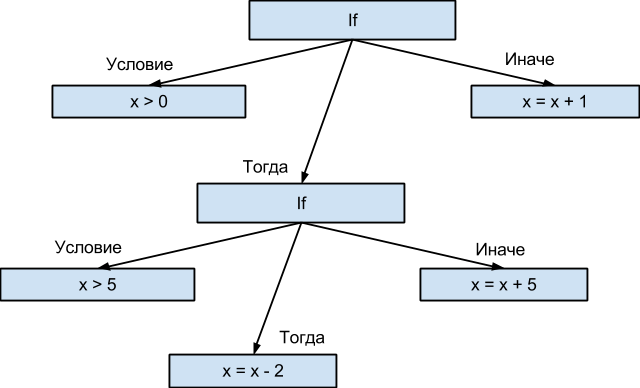
\includegraphics[width=0.6\textwidth]{nestedIf}
	\caption{Пример дерева “\lstinline{if-then-else}”}
	\label{fig:nestedIf}
\end{figure}

\begin{figure}[h!]
	\centering
	\lstinputlisting{codes/nestedIf.l}
	\caption{Представление с помощью шаблонов с рис. \ref{fig:ifTmplt}}
	\label{fig:nestedIfCode}
\end{figure}

Одним из неочевидных свойств шаблонов является то, что с их помощью можно выражать не только базовые конструкции языка.
Например, можно завести отдельный шаблон для случая, когда обе ветки конструкции “\lstinline{if-then-else}” представляют собой операторы “\lstinline{write}” (см. рис. \ref{fig:writeNestedInIf}). Если добавить такой шаблон, то пример дерева с рисунка~\ref{fig:nestedIf} получит новое представление (см. рис. \ref{fig:nestedIfNew}).

\begin{figure}[h!]
	\lstinputlisting{codes/writeNestedInIf.t}
	\caption{Пример задания шаблона для сложной конструкции}
	\label{fig:writeNestedInIf}
\end{figure}

\begin{figure}[h!]
	\lstinputlisting{codes/nestedIfNew.l}
	\caption{Представление дерева с рис. \ref{fig:nestedIf} с импользованием шаблона с рис. \ref{fig:writeNestedInIf}}
	\label{fig:nestedIfNew}
\end{figure}

\subsection{Построение образцов}

Для работы принтера неообходимо иметь возможность сравнивать синтаксическое представление шаблонов с деревом, которое печатается. Поэтому необходим синтаксический анализатор, который может разбирать шаблонные конструкции в рамках целевого языка. Удобным способом разработать данный анализатор является использование расширяемого синтаксического анализатора целевого языка. В результате работы расширенного анализатора получается набор образцов. В узлах синтаксического дерева, соответсвующих меткам шаблонов, хранится информация о положении метки внутри текста образца, чтобы на этапе печати документа знать, куда вставлять представления поддеревьев.

\newpage

\subsection{Печать дерева с использованием набора образцов}

На этапе, когда уже имеются необходимые образцы, происходит их сопоставление с синтаксическим деревом, переданным на печать. С помощью этого и происходит печать дерева.
Псевдокод алгоритма приведен ниже (см. рис. \ref{fig:comparePseudoCode}).

\begin{figure}[h!]
	\begin{algorithmic}
		\State{H --- ассоциативный массив, связывает деревья с их текстовым представлением}
		\State{M --- набор образцов для языковых конструкций}

		\Function{print}{$tree$} \Comment{По дереву строит его текстовое представление}
			\If{$tree \in H$}
				\State\Return{$H[tree]$}
			\Else
				\State{Вызов print для поддеревьев $tree$}
				\State\Return{\Call{templateIter}{$tree$}}
			\EndIf
		\EndFunction

		\Function{templateIter}{$tree$} \Comment{Перебирает все образцы и пытается их применить к дереву}
			\ForAll{$(templateTree, text) \in M$}
				\State{$list$ := \Call{templateCompare}{$tree, templateTree$}} \Comment{В случае исключения, переходит к новому элементу $M$}
				\State{$H[tree]$ := построенное представление для $tree$ по $list$ и $text$}
				\State\Return{$H[tree]$}
			\EndFor
		\EndFunction

		\Function{templateCompare}{$tree, templateTree$} \Comment{Получает список координат метки в тексте шаблона и представления соответствующего текстового представления поддерева}
			\If{$tree$ и $templateTree$ одного типа}
				\State{Вызвать $templateCompare$ для соответствующих поддеревьев}
				\State\Return{соединенный список результатов вызова для поддеревьев}
			\EndIf

			\If{$templateTree$ является меткой}
				\If{$H[tree]$ соответствует ограничениям метки}
					\State\Return{$[($координаты метки$, H[tree])]$}
				\Else
					\State{создать исключение}
				\EndIf
			\EndIf
		\EndFunction

		% \SetAlgoLined
		% \KwData{Дерево для печати (T), набор образцов (M)}

		% \ForEach{образца (tree, text) $\in$ M}{
		% 	\eIf{m }

		% 	\eIf{T и tree одного типа}{
		% 		выполнить алгоритм для поддеревьев T
		% 	}{
		% 		создать исключение
		% 	}
		% }


	\end{algorithmic}
	\caption{Псевдокод сопоставления дерева с набором образцов}
	\label{fig:comparePseudoCode}
\end{figure}

Из псевдокода видно, что в случае, если для какого-нибудь поддерева не найдется соотвествующий образец, то дерево невозможно будет напечатать. То есть множество образцов должно быть достаточным. Это естественное ограничение.

Попробуем оценить время работы алгоритма. Пусть $|M|$ --- количество образцов, $height(T)$ --- высота дерева, а $K$ --- максимальное число поддеревьев у узла синтаксического дерева целевого языка. Тогда время работы алгоритма можно оценить как $O((|M| \times K)^{height(T)} )$.

\subsection{Реализованный принтер}

Описанный подход был реализован в качестве принтера языка L на языке OCaml\footnote{http://ocaml.org}. Для написания синтаксического анализатора была использована библиотека Ostap\footnote{http://oops.math.spbu.ru/projects/ostap}.

